\section{Beschreibung der Implementierung}
Um die Funktionsweise der Softwarelösung zu verstehen, ist eine klare Übersicht über die einzelnen Bestandteile notwendig. Diese wird im Folgenden über ein Klassendiagramm inkl. Beschreibung gegeben. Danach werden noch die einzelnen Abschnitte in ihrer Funktion beschrieben.

\subsection{Klassendiagramm}
Bevor auf den genauen Funktionsablauf der Applikation eingegangen wird, sollte zuerst ein Überblick auf die Implementierung gegeben werden. Hierzu ist in Abbildung \ref{classDiagram} der komplette Umfang aller Klassen aufgezeigt
\footnote{Aus Gründen der Übersichtlichkeit wurden die getter- und setter-Methoden weggelassen, um die Abbildung nicht über zu dimensionieren}. Leicht erkennbar ist, dass der größte Teil der Logik innerhalb des aco-Pakets - welches unter anderem Ant und Colony enthält - stattfindet. Landscape, also die Klasse welche das \ac{TSP} beschreibt, dient nur als Schnittstelle zur Abfrage der Distanzen zwischen den Städten.

\begin{figure}[h]
	\centering
	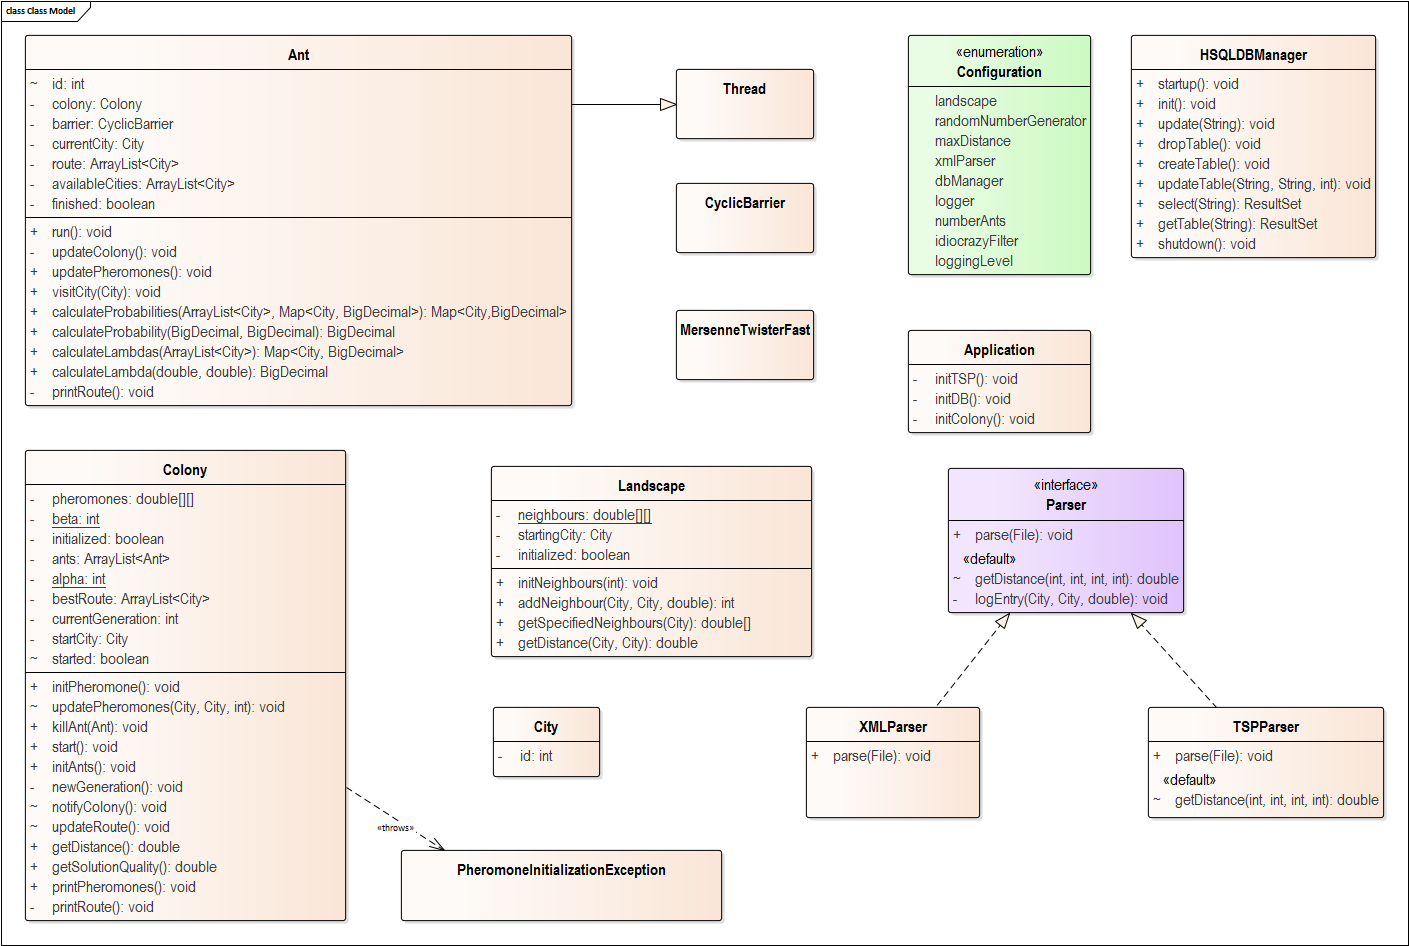
\includegraphics[width=\linewidth]{../../../01_uml/classModel.png}
	\caption{Klassendiagramm der vorliegenden Softwarelösung}
	\label{classDiagram}
\end{figure}

\subsection{Persistenz}
Um die Ergebnisse der einzelnen Generationen persistent abspeichern zu können, ohne den Speicherverbrauch des Programms ansteigen zu lassen, wird eine Datenbank-Anbindung an eine HSQLDB-Datenbank verwendet. Um die Performance möglichst hoch und den Datenbankumfang möglichst klein zu halten, werden in dieser allerdings nur zwei Tabellen erstellt und verwaltet.

\begin{figure}[h]
	\centering
	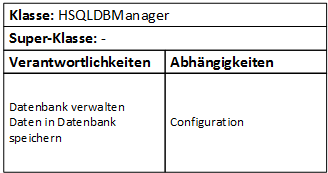
\includegraphics[width=0.4\linewidth]{images/CRC_persistenz.png}
	\caption{Modellierung der Klassen des Persistenz-Bereichs über CRC-Karten}
	\label{crcPersistenz}
\end{figure}


Zum Einen wird von jeder Generation, welche den Algorithmus durchlaufen hat, die beste Route erfasst und abgespeichert. Hierbei besteht ein Tabelleneintrag lediglich aus einer Zufalls-ID, der Route als String und der Distanz als Double. 

Zum Anderen wird eine Tabelle zur Verfolgung der Verbesserung angelegt. In der Historie wird eine Route nur dann abgespeichert, wenn diese sich im Vergleich zur vorherigen auch verbessert hat. Somit besteht diese aus den gleichen Attributen, wie die Generationen-Tabelle, mit dem Zusatz, dass auch die Generation, welche die Verbesserung verursacht hat, mit einer Ganzzahl abgespeichert wird.

\subsection{Applikation}
Dem Bereich der Applikation sind die Klassen zugeordnet, welche sich um die Initialisierung bzw. die Verwaltung von zentralen Parametern kümmern. Somit sind hier die Klassen Application, Configuration, sowie alle Implementierungen des Parser-Interfaces zu finden. In Abbildung \ref{crcApplikation} ist eine Modellierung dieser Klassen über CRC-Karten gezeigt.

Application ist beim Start des Programms dafür verantwortlich, dass alle wichtigen Instanzen korrekt initialisiert werden. Darunter fällt das Starten des Parsers, des HSQLDB-Managers, sowie der Ameisenkolonie. Sobald die Kolonie gestartet ist, ist die letzte Aufgabe der Application auf das Ende der Berechnung zu warten und dann die Datenbank wieder abbauen zu lassen.

Configuration ist als zentrale Anlaufstelle für alle Instanzen, die nur einmal benötigt werden, und alle Parameter, die mehrfach benötigt werden, gedacht. So verwaltet diese unter anderem die Gewichtung der Parameter bei der Berechnung der Wahrscheinlichkeiten. Auch wird über die Configuration der zentrale Logger bereitgestellt. Über diesen werden die Ergebnisse der Generationen erfasst bzw. auch Debug-Informationen gesammelt.

\begin{figure}[h]
	\centering
	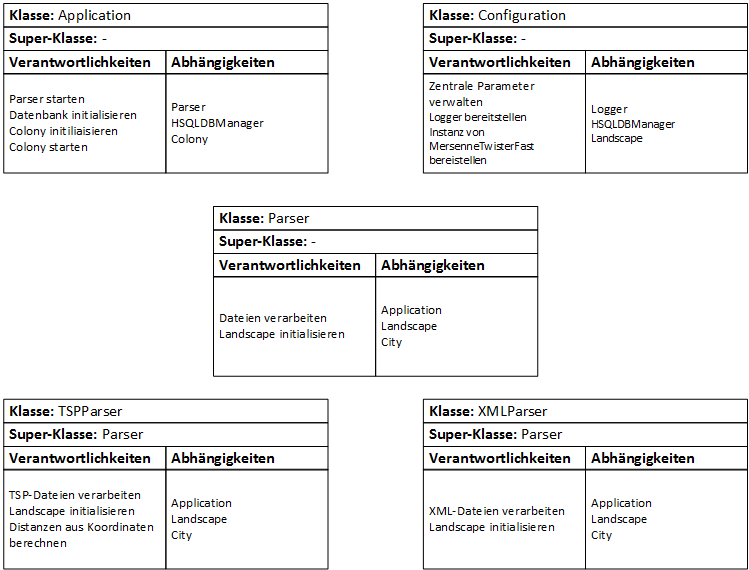
\includegraphics[width=\linewidth]{images/CRC_applikation.png}
	\caption{Modellierung der Klassen des Applikation-Bereichs über CRC-Karten}
	\label{crcApplikation}
\end{figure}

Alle Implementierungen des Parser-Interfaces haben einen gemeinsamen Zweck: Die Landscape-Klasse - welche auch von Configuration verwaltet wird - zu konfigurieren und die Problemstellung zu generieren. Hierzu gibt es zwei Varianten: Es kann entweder eine XML-Datei erstellt werden, welche eine bestimmte Formatierung erfüllen muss. Oder aber es kann eine \ac{TSP}-Datei beigefügt werden, welche dem Standard der \ac{TSP}-Problemstellungen folgt. In beiden Fällen wird die Datei ausgelesen und die Problemstellung in die Applikation importiert, sodass die Ameisenkolonie auf dieser aufbauen kann.

\subsection{TSP}
Der \ac{TSP}-Bereich der Architektur dient zu aller erst der Verdeutlichung des Aufbaus. So soll durch die Verwendung der City-Klasse statt einfachen Integern das Verständnis gefördert werden. Innerhalb der Landscape-Instanz - welche in der Konfiguration zentral initialisiert wird -  wird die zweidimensionale Matrix der Distanzen zwischen den Städten bereit gehalten. 

Über diese Matrix kann immer zentralisiert der Wert von den Ameisen nachgefragt werden, ohne eine unnötige Berechnung durchzuführen. Ebenso fördert dieser Aufbau die Sicherung der Funktionsfähigkeit, da einfacher sichergestellt werden kann, dass die Distanzen richtig berechnet werden. Ein weiterer Vorteil ist, dass die Ameisen hier eine Liste von Nachbarn der derzeitigen Position nachfragen können, indem sie ihren derzeitigen Standort übergeben. Dies vereinfacht das Konzept bei der Berechnung innerhalb der Ameisen-Klasse.

\begin{figure}[h]
	\centering
	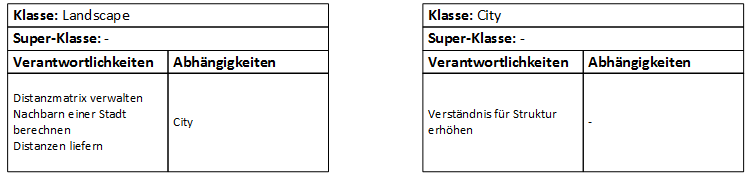
\includegraphics[width=\linewidth]{images/CRC_tsp.png}
	\caption{Modellierung der Klassen des \ac{TSP}-Bereichs über CRC-Karten}
	\label{crcTsp}
\end{figure}

\subsection{ACO}
Der hauptsächliche Teil der Berechnung wird innerhalb des \ac{ACO}-Bereichs durchgeführt. Denn hier befindet sich die Ameisenkolonie, als Verwaltungsorgan, und die Ameisen, welche als Threads gleichzeitig auf die Suche nach der bestmöglichen Lösung gehen.

\begin{figure}[h]
	\centering
	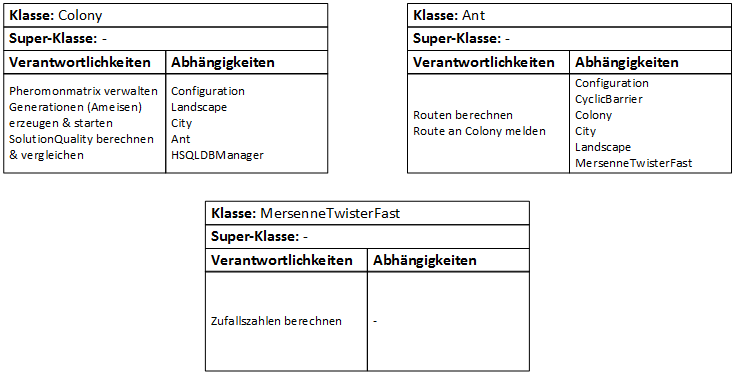
\includegraphics[width=\linewidth]{images/CRC_aco.png}
	\caption{Modellierung der Klassen des \ac{ACO}-Bereichs über CRC-Karten}
	\label{crcAco}
\end{figure}


Von der Kolonie werden die Ameisen insofern verwaltet, dass die Threads über diese Klasse gestartet werden, sowie hier auch die Ergebnisse abgeliefert werden. Nach jeder Generation wird innerhalb der Kolonie für jede Ameise eine Auswertung gestartet, ob die Route besser war als die derzeit beste. Sollte dies der Fall sein, wird die alte Route mit der neuen Route überschrieben.

Unabhängig davon ob eine neue beste Route gefunden wurd oder nicht, wird nach jeder Generation von Ameisen ein Update auf die Pheromonmatrix durchgeführt. Hierbei meldet jede Ameise für jeden Weg, den sie zwischen zwei Städten gegangen ist, einen Wert, welcher auf den derzeitigen Pheromonwert addiert werden soll. Hierfür iteriert eine Ameise über die Route, welche sie sich gemerkt hat, und ruft die updatePheromone-Methode der Kolonie auf, mit dem Wert $1/distance$, wobei $distance$ der Distanz zwischen der Stadt, über welche gerade iteriert wird, und der Folgestadt beträgt. 

Die restliche Berechnungsarbeit wird von den einzelnen Ameisen bzw. Threads bewältigt. Diese berechnen ab dem Startpunkt für alle möglichen Nachbarn
\footnote{Ein Nachbar ist dann erreichbar, wenn dieser noch nicht in der Route vorgekommen ist, also noch nicht besucht wurde.} einen $\lambda$-Wert\footnote{Beschrieben wurde diese Berechnung bereits in Kapitel \ref{parameter}}. 
Als nächstes werden alle $\lambda$s aufsummiert, um mit den einzelnen $\lambda$s der Städte dividiert durch die Summe die Wahrscheinlichkeit zu berechnen. Hierdurch wird beschrieben, dass Städtepaare, welche eine kurze Distanz besitzen, sowie einen hohen Pheromonwert besitzen, deutlich wahrscheinlicher besucht werden. Hierbei kann eine unterschiedliche Gewichtung vorgenommen werden, wie in Kapitel \ref{parameter} und Kapitel \ref{analyse} beschrieben wurde.

Nachdem für alle erreichbaren Städte die Wahrscheinlichkeiten berechnet wurden, wird eine Zufallszahl bestimmt. Sollte eine Wahrscheinlichkeit für eine Stadt höher sein, als die Zufallszahl so wird die Berechnung an dieser Stelle beendet und die Ameise besucht diese Stadt. Sollte diese Bedingung für keine einzelne Stadt erfüllt werden, so werden die Wahrscheinlichkeiten solange aufsummiert bis die Summe größer ist als die Zufallszahl. Die Stadt, bei welcher diese Schwelle überschritten wird, wird dann von der Ameise aufgesucht.

Sobald jede Ameise ihre Route beendet hat und wieder bei der Anfangsstadt angekommen ist, wird über die CyclicBarrier zentral eine Methode innerhalb der Kolonie angestoßen. Diese fordert nach und nach jede Ameise auf, das Ergebnis zu melden, um die Pheromonmatrix zu aktualisieren. Nachdem die Kolonie vollständig aktualisiert wurde, ist die derzeitige Generation beendet und es wird eine neue generiert und gestartet.